\documentclass[12pt, a4paper]{article}

% Idioma e codificação
\usepackage[utf8]{inputenc}
\usepackage[english]{babel}

% Layout e margens
\usepackage[top=3cm, bottom=2cm, left=3cm, right=2cm]{geometry}
\usepackage{parskip}
\linespread{1.0}

% Pacotes de matemática
\usepackage{amsmath, amsfonts, amssymb}
\usepackage{mathtools}

% Gráficos, tabelas e elementos flutuantes
\usepackage{graphicx}
\usepackage{float}
\usepackage{caption}
\usepackage{pdflscape}
\usepackage{caption}
\usepackage{subcaption}

% Listagem de código e gestão de cores
\usepackage{listings}
\usepackage{color}

% Diversos
\usepackage{enumitem}
\usepackage{indentfirst}
\usepackage{authblk}
\usepackage{hyperref}
\usepackage{booktabs}

\lstset{
    language= Python,
    basicstyle=\ttfamily\small,
    aboveskip={1.0\baselineskip},
    belowskip={1.0\baselineskip},
    columns=fixed,
    extendedchars=true,
    breaklines=true,
    tabsize=4,
    prebreak=\raisebox{0ex}[0ex][0ex]{\ensuremath{\hookleftarrow}},
    frame=lines,
    showtabs=false,
    showspaces=false,
    showstringspaces=false,
    keywordstyle=\color[rgb]{0.627,0.126,0.941},
    commentstyle=\color[rgb]{0.133,0.545,0.133},
    stringstyle=\color[rgb]{01,0,0},
    numbers=left,
    numberstyle=\small,
    stepnumber=1,
    numbersep=10pt,
    captionpos=t,
    escapeinside={\%*}{*)}
}

%%%%%%%%%%%%%%%%%%%%%%%%%%%%%%%%%%%%%%%%%%%%%%%%%%%%%%%%%%%%%%%%%%%%%%%%%%%%%%%%%

\title{A Numerical Analysis of the Lorenz Attractor}

\author{Julio Cezar de Moura Lima \and Lucas Amaral Taylor}
\date{2024}
\begin{document}

\maketitle

%%%%%%%%%%%%%%%%%%%%%%%%%%%%%%%%%%%%%%%%%%%%%%%%%%%%%%%%%%%%%%%%%%%%%%%%%%%%%%%%%
%%%%%%%%%%%%%%%%%%%%%%%%%%%%%%%%%%%%%%%%%%%%%%%%%%%%%%%%%%%%%%%%%%%%%%%%%%%%%%%%%

\begin{abstract}
	\begin{center}
		This report applies numerical methods to the system of differential equations of the Lorenz attractor.
		
		\vspace{0.25cm}
		
		\noindent \textbf{Keywords:} Numerical methods; Lorenz attractor;
	\end{center}
\end{abstract}


    
%%%%%%%%%%%%%%%%%%%%%%%%%%%%%%%%%%%%%%%%%%%%%%%%%%%%%%%%%%%%%%%%%%%%%%%%%%%%%%%%%
%%%%%%%%%%%%%%%%%%%%%%%%%%%%%%%%%%%%%%%%%%%%%%%%%%%%%%%%%%%%%%%%%%%%%%%%%%%%%%%%%
    
\section{Introduction}\label{introduction}

Edward Norton Lorenz (1917–2008) was a mathematician and meteorologist who made significant contributions to the study of weather forecasting using differential equations. The \textbf{Lorenz Attractor} was one of his most important contributions in this field. Published in the journal \textit{Journal of the Atmospheric Sciences} in 1963 under the title \textit{Deterministic Nonperiodic Flow} \cite{Lorenz1963}, Lorenz developed a simplified mathematical model for atmospheric convection, consisting of three ordinary differential equations shown below:

\begin{align}
	\begin{cases}
	\dfrac{dx}{dt} & = \sigma(y-x)     \\
	\dfrac{dy}{dt} & = x(\rho - z) - y \\
	\dfrac{dz}{dt} & = xy - \beta z    
	\end{cases}
	\label{eq:apresentacao-sistema}
\end{align}

In addition to its clear importance to meteorology, the model is known for being chaotic and for initiating the study of Chaos Theory.

In this report, following the footsteps of Edward Norton Lorenz as well as Ellen Cole Fetter Gille and Margaret Elaine Hamilton — two important mathematicians who contributed to Lorenz's work — we will perform numerical simulations to study the system of equations shown in \eqref{eq:apresentacao-sistema}.

Naturally, our work is at the undergraduate level and, as instructed, makes use of the content covered in class. For this task, we will follow the following approach: first, we will use the \textit{Runge-Kutta} method to discretize and solve the differential equation system that defines the attractor. Then, for graphical representation, we will use \textit{cubic splines}. The Lorenz attractor has smooth curves, and we believe this is the most appropriate method for visualizing them. Finally, we will apply the Least Squares Method (LSM) to assess the sensitivity of the system (which is known to be highly sensitive). With LSM, we will generate a set of simulations with slight variations in each parameter and compare the results.

    
\newpage
\section{Mathematical Modeling}

In this section, we present the assumptions and considerations that lead to the differential equation modeling the system. In addition, we show how the system of equations is consistent with the Cauchy Problem, and finally, we present the initial conditions and the problem's domain of definition.

\subsection{Assumptions and Considerations}

In the introduction of his article, Lorenz states that the system of equations shown in \eqref{eq:apresentacao-sistema} is a deterministic model of ideal hydrodynamic systems, and that such systems were developed to represent a dissipative forced hydrodynamic system. Furthermore, it is important to highlight that the work in the article \textit{Deterministic Nonperiodic Flow} \cite{Lorenz1963} is primarily based on the article \textit{Finite Amplitude Free Convection as an Initial Value Problem—I} published in 1962 by Barry Saltzman \cite{Saltzman1962}.

Based on Saltzman's article, we introduce to the reader the meteorological concepts, the methodology used by the author, and finally the mathematical reasoning that leads from the equations proposed by Saltzman to the system in \eqref{eq:apresentacao-sistema} as studied by Lorenz. The details of the equation's derivation can be consulted in the cited references \cite{Lorenz1963} and \cite{Saltzman1962}.

Before proceeding, it is necessary to explain the phenomenon of convection. Convection is a process of heat transfer that occurs in fluids, such as liquids and gases. This phenomenon involves the movement of the fluid itself, transferring thermal energy from one region to another.

In \cite{Saltzman1962}, the author bases his work on meteorological and hydrodynamic experiments. In these, researchers worked with models of a convection phenomenon of nonlinear nature, due to spatial variations in motion and temperature. Saltzman had two objectives: to formulate a mathematical model and a solution method for a time-dependent two-dimensional convective flow case. For this, he used a fixed and limited number of Fourier components and results from previous works, notably: \textit{On convection currents in a horizontal layer of fluid, when the higher temperature is on the under side} \cite{Rayleigh1916} and \textit{Ueber die Wärmeleitung der Flüssigkeiten bei Berücksichtigung der Strömungen infolge von Temperaturdifferenzen} \cite{Oberbeck1879}.

After some algebraic manipulations (whose details can be found in \cite{Saltzman1962}), Saltzman arrives at the following system of differential equations:

\begin{align}
	\frac{\partial}{\partial t} \nabla^2 \psi & = - \frac{\partial (\psi, 
	\nabla^2 \psi)}{\partial (x,z)} + v \nabla^4 \psi + g \alpha
	\frac{\partial \theta}{\partial x} \label{saltzman-1}                                \\
	\frac{\partial}{\partial t} \theta        & = \frac{\partial (\psi,   
	\theta)}{\partial (x,z)} + \frac{\Delta T}{H} \frac{\partial \psi}{\partial x}
	+ \kappa \nabla^2 \theta \label{saltzman-2}
\end{align}

Where:
\begin{itemize}
	\item $\psi$: stream function (m$^2 \cdot$ s$^{-1}$);
	\item $\theta$: temperature deviation (K);
	\item $g$: gravitational acceleration (m $\cdot$ s$^{-2}$);
	\item $\alpha$: thermal expansion coefficient (K$^{-1}$);
	\item $v$: kinematic viscosity constant (m$^2 \cdot$ s$^{-1}$);
	\item $\kappa$: thermal conductivity constant (W $\cdot$ m$^{-1} \cdot$ K$^{-1}$).
\end{itemize}

Manipulating the terms and introducing Fourier components, we obtain the following expressions \cite{peitgen2013} \cite{Saltzman1962}:

\begin{align}
	\frac{a}{(1 + a^2)^k} \psi        & = x(t)\sqrt{2} \sin \left(\frac{\pi 
	u}{a}\right) \sin \left(\frac{\pi v}{H}\right) \label{saltzman-forier-1} \\
	\frac{\pi R_o \theta}{R \Delta T} & = y(t)\sqrt{2} \cos \left(\frac{\pi 
	u}{a}\right) \sin \left(\frac{\pi v}{H}\right)
	\label{saltzman-forier-2} - z(t)
	\sin \left(\frac{2\pi}{H}v\right)
\end{align}

Where:
\begin{itemize}
	\item $u$: horizontal spatial coordinate (m);
	\item $x(t), y(t), z(t)$: time-dependent coefficients (amplitudes) (units depend on context);
	\item $\frac{\pi}{H}$: inverse of the fluid layer depth (maximum of $v$) (m$^{-1}$);
	\item $a$: geometric parameter;
	\item $Ra$: Rayleigh number \cite{Rayleigh1916};
	\item $R_c$: critical value of $Ra$ ($R_c = \pi^4(1 + a^2)^3/a^2$);
	\item $\Delta T$: total temperature difference (K).
\end{itemize}

Finally, with all these equations at hand, by substituting \ref{saltzman-forier-1} and \ref{saltzman-forier-2} into \ref{saltzman-1} and \ref{saltzman-2}, and eliminating the trigonometric functions, we obtain \ref{eq:apresentacao-sistema}, that is:

\begin{align*}
	\begin{cases}
	\dfrac{dx}{dt} & = \sigma(y - x)   \\
	\dfrac{dy}{dt} & = x(\rho - z) - y \\
	\dfrac{dz}{dt} & = xy - \beta z    
	\end{cases}
\end{align*}

\begin{itemize}
	\item $\sigma$ controls the system's sensitivity to the difference between variables $x$ and $y$ (Prandtl number).
	\item $\rho$ is associated with the convection rate of the system (Rayleigh number).
	\item $\beta$ is related to the system's geometry and the difference in the growth rates of variables $x$ and $z$.
\end{itemize}

\subsection{The Cauchy Problem}

In his article, Lorenz considers the system of equations as a dissipative energy system composed of a finite set of linear equations in phase space.

\subsubsection{A Dissipative System in Phase Space}

First, it is important to define what a dissipative energy system is, what phase space is, and how these concepts relate to the Lorenz attractor.

Dissipative systems are characterized by energy loss in non-conservative processes, such as friction, with energy being converted into less useful forms, such as heat. The Lorenz Attractor is one such example, as it models atmospheric convection (explained in the previous section), where energy is continuously input and dissipated.

Phase space is a representation that describes all possible states of a dynamical system using its variables. Each point in this space represents a specific state of the system.

That said, we can explain Lorenz's approach to demonstrating the existence and uniqueness of the differential equation's solution. The convection phenomenon can be modeled as a dissipative energy system composed of a finite set of linear equations. Thus, we consider $n$ variables $x_1, \ldots, x_n$ and define the following system:

\begin{equation}
	\frac{dx_i}{dt} = F_i\left(x_1, \ldots, x_n\right) \quad i \in \{1, \ldots, n\}
\end{equation}

Where $F_i$ has continuous first-order partial derivatives and $t$ is the only independent variable. Therefore, to describe all possible states of a dynamical system using its variables, we model the system in an $n$-dimensional Euclidean phase space composed of the variables $x_1, \ldots, x_n$.

Since the system is composed of linear equations with dependent variables and $F_i \in C^1$, it consequently admits a unique solution. That is:

\begin{equation}
	x_i = f_i(x_{1_0}, \ldots, x_{n_0}, t) \quad i = \{1, \ldots, n\}
\end{equation}

For some interval containing $t_0$ and satisfying the condition below:

\begin{equation*}
	f_i(x_{1_0}, \ldots, x_{n_0}, t_0) = x_{i_0} \quad i = \{1, \ldots, n\}
\end{equation*}

This fact is demonstrated in \cite{ford1933} in the form of the following theorem:

\textbf{Theorem.} Consider a closed interval $[A, B]$ where the functions $F_i(x_1, \ldots, x_n)$ are continuous along with their first-order partial derivatives $\frac{\partial F_i}{\partial x_j}$ for all $1 \leq i,j \leq n$. If for some point $t_0$ in $(A, B)$ initial conditions $x_{i_0} = x_i(t_0)$ are given, then there exists a unique set of functions $x_i(t)$ that are solutions to the system in the interval $[A, B]$ and satisfy $x_i(t_0) = x_{i_0}$. Furthermore, the solutions $x_i(t)$ have continuous derivatives in $[A, B]$.

Based on the theorem above and the formulation of the differential equations $\frac{dx_i}{dt} = F_i(x_1, \ldots, x_n)$, the \textit{Cauchy} problem is properly satisfied. Given initial conditions at some time $t_0$, the existence and uniqueness of the solutions $x_i(t)$ are guaranteed in the interval $[A, B]$.

\subsubsection{A Brief Note on the Picard Existence and Uniqueness Theorem}

First, we state the Picard Existence and Uniqueness Theorem as in \cite{sotomayor1979}:

\textbf{Theorem.} Let $f$ be continuous and Lipschitz on $\Omega = I_a \times B_b$, where $I = \{t; \left|t - t_0 \right| \leq a\}$, $B_b = \{x; \left|x - x_0 \right| \leq b\}$. If $|f| \leq M$ on $\Omega$, then there exists a unique solution to

\begin{equation*}
	x^\prime = f(t, x), \quad x(t_0) = x_0
\end{equation*}

on $I_\alpha$, where $\alpha = \min \{a, b/M\}$.

In general, the theorem above is used to demonstrate the resolution of the \textit{Cauchy} problem. However, this method was not used for the Lorenz system.

After consulting books and references on the subject, none used this approach. Although it is easy to demonstrate that the functions in system \eqref{eq:apresentacao-sistema} have continuous derivatives, proving that the system is locally Lipschitz is extremely complex due to its nonlinearity. Therefore, the approach taken by the original author in \cite{Lorenz1963} is preferred. We chose to follow this widely adopted approach.

\subsubsection{Initial Conditions and Problem Domain}
\label{sec:cond-ini}

We define the problem's domain as follows: the variables $x, y, z \in \mathbb{R}$ reflect the system's ability to reach any state in three-dimensional space (note: although Lorenz treats the system in phase space, for simplicity and clarity in computational representation, we use the three-dimensional space in our simulations). In addition, we assume $t \in [0, \infty)$ — time starts at zero and has no upper bound, allowing the system to be analyzed dynamically over time.
	
	The initial conditions we define are: $\sigma = 10$, $\rho = 28$, and $\beta = \frac{8}{3}$. These values are typically chosen in simulations in the literature. Furthermore, the initial values of $x$, $y$, and $z$ are arbitrarily selected real numbers; for simplicity, we choose: $x = 0$, $y = 1.0$, and $z = 1.05$.
	\newpage
	
	%%%%%%%%%%%%%%%%%%%%%%%%%%%%%%%%%%%%%%%%%%%%%%%%%%%%%%%%%%%%%%%%%%%%%%%%%%%%%%%%%
	%%%%%%%%%%%%%%%%%%%%%%%%%%%%%%%%%%%%%%%%%%%%%%%%%%%%%%%%%%%%%%%%%%%%%%%%%%%%%%%%%
	
	\section{Numerical Methodology}
	
	In this section, we present the methods used in the development of this work, properly justifying the use of each one. For a proper description of each method, we refer to \cite{roma2023} and \cite{burden2016}.
	
	\subsection{A Brief Note on the Methods Used}
	
	Here, we present the numerical methods from a theoretical perspective, detailing the justification and functioning of each method according to the approach adopted in class. It is important to note that, in practical applications, we used the \textit{numpy} and \textit{scipy} libraries in the \textit{Python} programming language. We chose not to include in the text certain discrepancies and technical details related to the use of these tools, as they pertain more to implementation aspects of the libraries than to the theoretical concepts discussed in class.
	
	\subsection{Runge-Kutta Method}
	\subsubsection{Justification for the Choice of Method}
	
	The Lorenz attractor is a nonlinear and highly sensitive system, especially with respect to changes in initial conditions, and exhibits chaotic behavior. Since the method calculates slopes at four points within each time interval, it provides a more accurate approximation compared to the other methods studied in class. For instance, the Euler method would not be effective enough for discretizing the system, as it does not adequately model nonlinear phenomena.
	
	Moreover, the fourth-order Runge-Kutta method provides a local truncation error of order $h^5$ and a global truncation error of order $h^4$, where $h$ is the time step \cite{burden2016} \cite{roma2023}. This means that small increases in the time step can still yield accurate results without significantly increasing the error, making it ideal for handling the complex and sensitive dynamics of the Lorenz attractor.
	
	\subsubsection{Method Description}
	
	The Runge-Kutta method is used to discretize the values of the system \eqref{eq:apresentacao-sistema} given the initial values presented in Section \ref{sec:cond-ini}. We follow the formulation given in \cite{roma2023}:
	
	\begin{equation}
		\Phi(t, y, h) = \frac{1}{6} (\kappa_1 + 2\kappa_2 + 2\kappa_3 + \kappa_4)
	\end{equation}
	
	Where:
	\begin{align}
		\begin{cases}                                                     
		\kappa_1 = f(t, y)                                                \\
		\kappa_2 = f\left(t + \frac{h}{2}, y + \frac{h}{2}\kappa_1\right) \\
		\kappa_3 = f\left(t + \frac{h}{2}, y + \frac{h}{2}\kappa_2\right) \\
		\kappa_4 = f(t + h, y + h\kappa_3)                                
		\end{cases}                                                       
	\end{align}
	
	\subsection{Cubic Spline}
	\subsubsection{Justification for the Choice of Method}
	
	We use the cubic spline interpolation method. The choice of this method for interpolating the Lorenz attractor data is motivated by the need to represent the system’s curves in a smooth and continuous manner—an essential feature for handling its nonlinear and chaotic nature.
	
	Other methods, such as Lagrange interpolation, would not be suitable since they involve a linearization process that could lead to information loss, and therefore would not represent the system as accurately as desired.
	
	\subsubsection{Method Description}
	
	This method involves creating a cubic polynomial in each subinterval of a given total interval to interpolate a set of given data points. We follow the spline construction proposed in \cite{burden2016}, expressed below:
	
	Let $f$ be a function defined on the interval $[a,b]$ and $ \{a = x_0 < x_1 < \ldots < x_n = b\}$ a set of nodes. A cubic spline interpolant $S$ for $f$ is a function that satisfies the following conditions:
	
	\begin{enumerate}
		\item $S(x)$ is a cubic polynomial, denoted $S_j(x)$, on each subinterval $[x_j, x_{j+1}]$, for $j = 0, 1, \ldots, n-1$.
		\item $S_j(x_j) = f(x_j)$ and $S_j(x_{j+1}) = f(x_{j+1})$ for each $j = 0, 1, \ldots, n-1$.
		\item $S_{j+1}(x_{j+1}) = S_j(x_{j+1})$ for each $j = 0, 1, \ldots, n-2$.
		\item $S'_{j+1}(x_{j+1}) = S'_j(x_{j+1})$ for each $j = 0, 1, \ldots, n-2$.
		\item $S''_{j+1}(x_{j+1}) = S''_j(x_{j+1})$ for each $j = 0, 1, \ldots, n-2$.
		\item One of the following boundary conditions is satisfied:
		      \begin{enumerate}
		      	\item $S''(x_0) = S''(x_n) = 0$ (natural boundary condition).
		      	\item $S'(x_0) = f'(x_0)$ (clamped boundary condition).
		      \end{enumerate}
	\end{enumerate}
	
	\subsection{Least Squares Method}
	\subsubsection{Justification for the Choice of Method}
	
	We use the Least Squares Method (LSM) to analyze the sensitivity of the Lorenz attractor over time. Although the Lorenz attractor is a highly nonlinear system, LSM provides a good approximation of the system’s dynamics. In addition, it quantifies the impact of changes in each parameter, showing how small variations in the variables can affect the system. Finally, the method is also computationally efficient.
	
	\subsubsection{Method Description}
	
	The polynomial least squares method approximates a set of data points $(x_i, y_i)$ with an algebraic polynomial $P_n(x)$ of degree $n < m - 1$, choosing the coefficients $a_0, a_1, \ldots, a_n$ to minimize the quadratic error $E = \sum_{i=1}^m (y_i - P_n(x_i))^2$. This leads to $n + 1$ normal equations for the $n + 1$ unknown coefficients $a_j$:
	
	\begin{equation}
		\sum_{k=0}^n a_k \left(\sum_{i=1}^m x_i^{j+k}\right) = \sum_{i=1}^m y_i x_i^j,
		\quad \text{for each } j = 0, 1, \ldots, n.
	\end{equation}
	
	Solving this system gives the coefficients of the polynomial that best fits the data in the least squares sense, expressed as:
	
	\begin{equation*}
		P_n(x) = a_nx^n + a_{n-1}x^{n-1} + \cdots + a_1x + a_0
	\end{equation*}
	
	Details can be found in \cite{burden2016}.
	\newpage
	
	    
	%%%%%%%%%%%%%%%%%%%%%%%%%%%%%%%%%%%%%%%%%%%%%%%%%%%%%%%%%%%%%%%%%%%%%%%%%%%%%%%%%
	%%%%%%%%%%%%%%%%%%%%%%%%%%%%%%%%%%%%%%%%%%%%%%%%%%%%%%%%%%%%%%%%%%%%%%%%%%%%%%%%%
	    
	\section{Computational Methodology}
	
	In order to apply the methods previously discussed, this section aims to present the computational approach used to implement the methods, demonstrate the attractor behavior, and finally evaluate some metrics derived from each methodology.
	
	\subsection{Context}
	
	We present "discretization" methods that allow us to estimate values for the solution vector $S = \begin{bmatrix} x(t) \\ y(t) \\ z(t)\end{bmatrix}$ at a given time $t$. During the computational methodology, the following steps were carried out:
	
	\begin{enumerate}
		\item Application of the Runge-Kutta method to the Lorenz system with $n\_steps = 10^4$, meaning the solution vector is computed over 10,000 time steps. The justification for the number of steps is given graphically, as the attractor takes shape over time.
		\item From the RK solutions obtained, the data are tabulated and then used for cubic spline interpolation. Similarly, for LSM (Least Squares Method), two interpolating polynomials are constructed.
		\item With the interpolating polynomials previously computed, we generate the corresponding plots.
	\end{enumerate}
	
	\subsection{Preliminary Data}
	
	Using the RK method, three simulations were performed for the already defined Lorenz system, showing that the attractor forms spirals according to the time steps. A larger time interval ($t$) provides better visualization of the attractor behavior as evidenced by Lorenz (\textit{see Figure \ref{fig:lorenz-comparativo}}).
	
	The \textit{Python} function responsible for computing RK is defined by the following parameters: $\sigma,\ \rho,\ \beta,\ x_0,\ y_0,\ z_0,\ h,\ \text{num\_steps}$. These correspond to the conventional system variables, where $(x_0,\ y_0,\ z_0)$ are the initial conditions and $h$ is the length of the time interval in which $t$ is evaluated.
	
	During function execution, common values used in Lorenz's studies were adopted:
	
	\begin{equation}
		\begin{aligned}
			\sigma            & = 10,          \\
			\rho              & = 28,          \\
			\beta             & = \frac{8}{3}, \\
			x_0               & = 0,           \\
			y_0               & = 1,           \\
			z_0               & = 1.05,        \\
			h                 & = 0.01,        \\
			\text{num\_steps} & = 10^4         
		\end{aligned}
	\end{equation}
	
	\begin{table}[H]
		\centering
		\begin{tabular}{|c|c|c|c|c|}
			\hline
			Index & X        & Y        & Z        \\
			\hline
			0     & 0.000000 & 1.000000 & 1.050000 \\
			1     & 0.095105 & 1.003039 & 1.022849 \\
			2     & 0.182649 & 1.030512 & 0.997333 \\
			3     & 0.265581 & 1.080595 & 0.973428 \\
			4     & 0.346436 & 1.152210 & 0.951187 \\
			5     & 0.427432 & 1.244918 & 0.930735 \\
			6     & 0.510567 & 1.358849 & 0.912268 \\
			7     & 0.597683 & 1.494637 & 0.896062 \\
			8     & 0.690531 & 1.653393 & 0.882484 \\
			9     & 0.790823 & 1.836671 & 0.872011 \\
			10    & 0.900278 & 2.046464 & 0.865257 \\
			11    & 1.020660 & 2.285199 & 0.863005 \\
			12    & 1.153819 & 2.555743 & 0.866250 \\
			13    & 1.301723 & 2.861417 & 0.876253 \\
			14    & 1.466492 & 3.206010 & 0.894607 \\
			15    & 1.650427 & 3.593802 & 0.923322 \\
			\hline
		\end{tabular}
		\caption{Selection of 15 points}
	\end{table}
	
	\begin{figure}[H]
		\centering
		\begin{subfigure}{0.32\textwidth}
			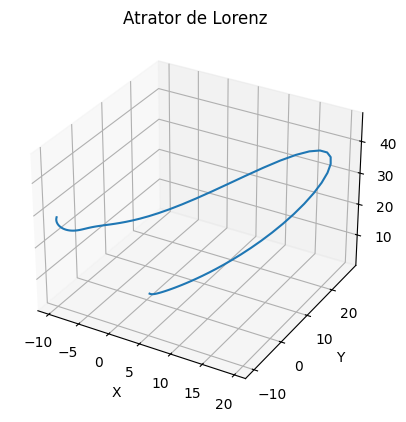
\includegraphics[width=\linewidth]{img/attrator100.png}
			\caption{100 steps}
			\label{fig:lorenz100}
		\end{subfigure}
		\hfill
		\begin{subfigure}{0.32\textwidth}
			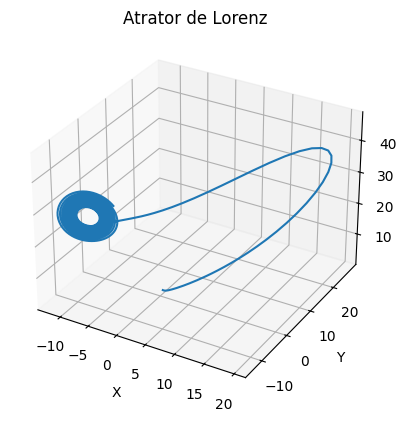
\includegraphics[width=\linewidth]{img/attrator1000.png}
			\caption{1000 steps}
			\label{fig:lorenz1000}
		\end{subfigure}
		\hfill
		\begin{subfigure}{0.32\textwidth}
			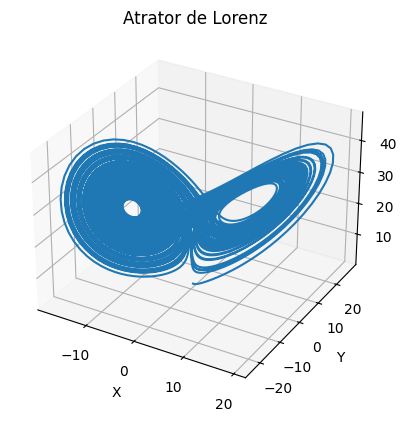
\includegraphics[width=\linewidth]{img/attrator10000.png}
			\caption{10000 steps}
			\label{fig:lorenz10000}
		\end{subfigure}
		\caption{Lorenz attractor trajectories for different numbers of steps.}
		\label{fig:lorenz-comparativo}
	\end{figure}
	
	\subsection{Interpolation Methods}
	
	\subsubsection{Cubic Spline}
	
	To implement the cubic spline interpolation method, we used the
	\href{https://docs.scipy.org/doc/scipy/index.html}{SciPy} library in Python, specifically the function
	\texttt{scipy.interpolate.CubicSpline}. This technique was chosen for testing and validation purposes,
	given the large number of data points involved, which results in a significant computational cost.
	Upon analyzing the method, we observe that its strategy aligns with the patterns already noted by
	Lorenz in his tests, making it a suitable interpolation method for capturing the "oscillatory"
	behavior described in the system.
	
	\begin{figure}[H]
		\centering
		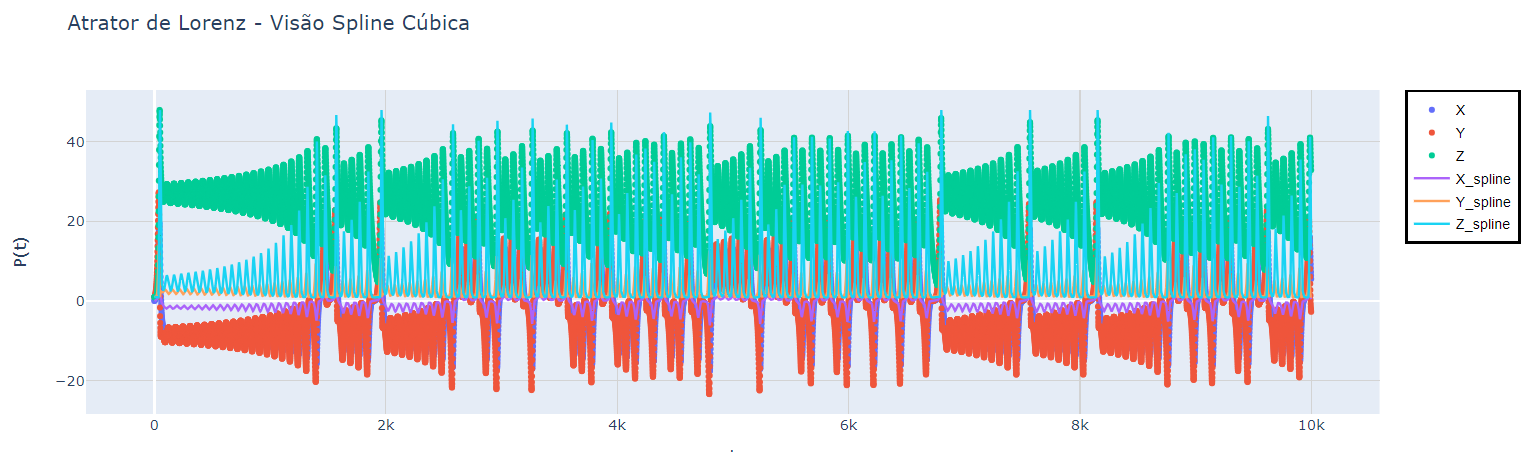
\includegraphics[width=\textwidth]{img/spline.png}
		\caption{Cubic Spline}
		\label{fig:spline}
	\end{figure}
	
	\subsubsection{Least Squares Method (LSM)}
	
	For the LSM, we followed the same strategy used with cubic splines, but instead employed the
	\href{https://numpy.org/doc/stable/index.html}{NumPy} library, specifically the \texttt{numpy.polyfit} function.
	This package performs a polynomial fit using the least squares approach based on the previously tabulated data points.
	In practice, the LSM does not provide a good curve fit, as it behaves more like linear regression,
	due to the high dispersion of the points, the large dataset size, and the resulting interpolation granularity.
	
	\begin{figure}[H]
		\centering
		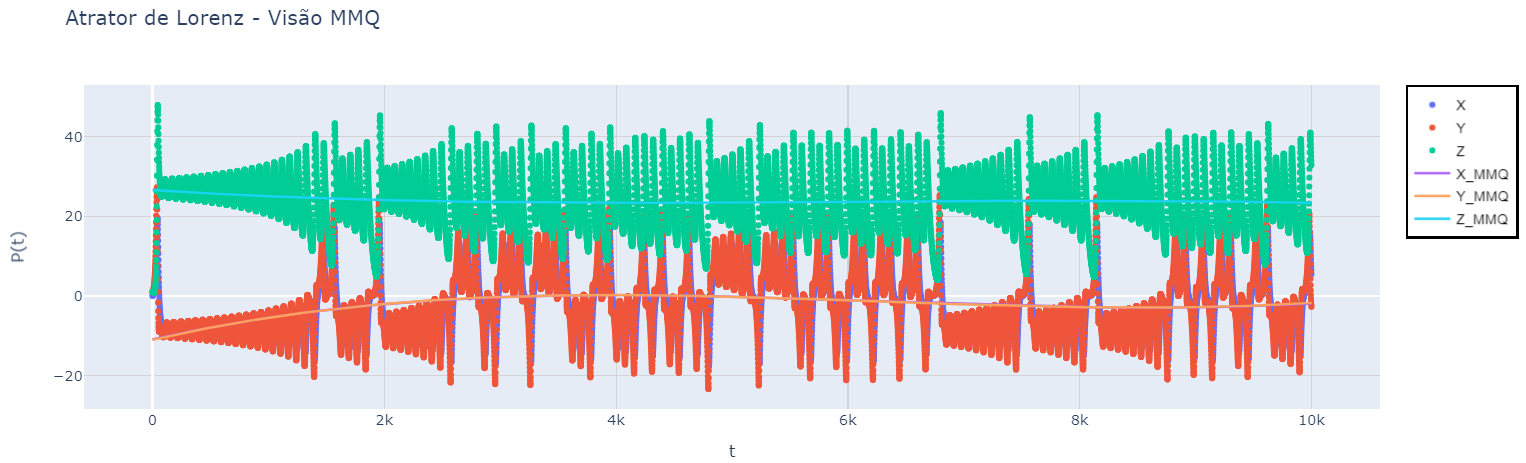
\includegraphics[width=\textwidth]{img/mmq.png}
		\caption{Least Squares Method (LSM)}
		\label{fig:mmq}
	\end{figure}
	
	\newpage
	
	    
	%%%%%%%%%%%%%%%%%%%%%%%%%%%%%%%%%%%%%%%%%%%%%%%%%%%%%%%%%%%%%%%%%%%%%%%%%%%%%%%%%
	%%%%%%%%%%%%%%%%%%%%%%%%%%%%%%%%%%%%%%%%%%%%%%%%%%%%%%%%%%%%%%%%%%%%%%%%%%%%%%%%%
	    
	\section{Results}
	\subsection{Manufactured Analysis}
	
	To conduct the analysis in a manufactured way, we present an intrinsic comparison between one of the methods used by Lorenz to solve the problem—the forward-difference method \cite{Lorenz1963}—and the method previously detailed in this text, namely the fourth-order Runge-Kutta method (RK4).
	
	For didactic purposes, let us outline the forward-difference method. The equation that defines the method is given by:
	\begin{equation*}
		X_i(t_{n+1}) = X_i(t_n) + F_i(P_n)\Delta t
	\end{equation*}
	where $F_i(P_n) = \dot X_i(P_n)$ and $t_{n+1} = t_n + \Delta t$. Thus, we use progressive approximations—i.e., finite differences applied to the function at a given time $t_n$ and at the next time step $t_{n+1}$—to estimate future values. Below we present the table of values generated using the forward-difference method, along with the pointwise differences compared to those obtained using RK4.
	
	    
	\begin{table}[H]
		\centering
		\begin{tabular}{|c|c|c|c|c|c|c|}
			\hline
			   & X        & Y        & Z        & $X-X_{rk}$ & $Y-Y_{rk}$ & $Z-Z_{rk}$ \\
			\hline
			1  & 0.000000 & 1.000000 & 1.050000 & 0.000000   & 0.000000   & 0.000000   \\
			2  & 0.100000 & 0.990000 & 1.022000 & 0.004895   & -0.013039  & -0.000849  \\
			3  & 0.189000 & 1.007078 & 0.995737 & 0.006351   & -0.023434  & -0.001596  \\
			4  & 0.270808 & 1.048045 & 0.971087 & 0.005226   & -0.032550  & -0.002341  \\
			5  & 0.348532 & 1.110761 & 0.948030 & 0.002096   & -0.041449  & -0.003157  \\
			6  & 0.424755 & 1.193938 & 0.926620 & -0.002678  & -0.050980  & -0.004114  \\
			7  & 0.501673 & 1.296994 & 0.906982 & -0.008894  & -0.061854  & -0.005286  \\
			8  & 0.581205 & 1.419943 & 0.889302 & -0.016478  & -0.074694  & -0.006760  \\
			9  & 0.665079 & 1.563312 & 0.873840 & -0.025452  & -0.090081  & -0.008644  \\
			10 & 0.754902 & 1.728089 & 0.860935 & -0.035921  & -0.108582  & -0.011076  \\
			\hline
		\end{tabular}
		\caption{Difference compared to the values of the RK4 points}
		\label{tab:rk44-diff}
	\end{table}
	\subsection{Sample Mean Analysis}
	
	Let $E = \left\{(\mu_x, \mu_y, \mu_z) \in \mathbb{R}^3\right\}$ be the vector of sample means of the absolute difference between corresponding points. Then $E = (0.007, 0.049, 0.004)$. From this, we can statistically observe that the generated points do not differ significantly in magnitude. However, due to the sensitive nature of the attractor, the graphical differences are substantial. We notice that the jumps at each iteration are smaller compared to RK4, which directly affects the attractor formation, resulting in more compact “vortices” and less detailed dynamics. The following figure illustrates this:
	
	\begin{figure}[H]
		\centering
		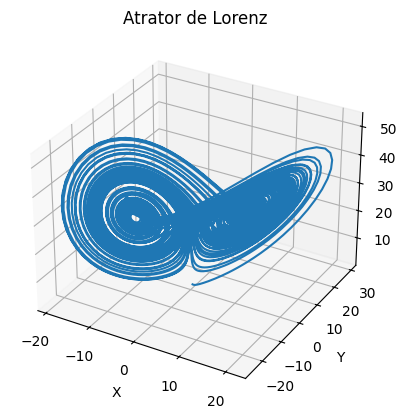
\includegraphics[width=0.4\textwidth]{img/attrator10000_lorenz.png}
		\caption{Image generated with the forward-difference method}
		\label{fig:diff-prog}
	\end{figure}
	
	\subsection{Applications in Meteorology}
	
	As previously stated in the introduction of this report, the importance of the Lorenz attractor in meteorology can be reaffirmed. Although it is a simplified model based on the one proposed by Saltzman in \cite{Saltzman1962}, Lorenz’s model is considered a robust tool for modeling atmospheric convection around the globe.
	
	A prominent example of its use is found in the work of Timothy Noel Palmer, titled “Extended-Range Atmospheric Prediction and the Lorenz Model” \cite{Palmer1993}, which we summarize below in a freely translated excerpt:
	
	\begin{quote}
		\fontsize{10}{12}\selectfont
		The physical basis for long-range forecasting is explored using the well-known three-component Lorenz convection model, taken as a conceptual representation of chaotic extratropical circulation, and extended by coupling it with a linear oscillator to represent large-scale tropical-extratropical interactions. The model is used to analyze the roles of time averaging and ensemble forecasting, and in an extended form, the impact of anomalous sea surface temperatures in both tropical and extratropical regions. The conceptual paradigms and analytical calculations presented are used to interpret results from numerical weather forecasts and general circulation model experiments. Observations are made on the relevance of predictability studies to the problem of climate change.
	\end{quote}
	
	    
	    
	\subsection{Forward-Difference Method}
	\subsubsection{Theoretical Foundation}
	
	The forward-difference method used in the manufactured analysis corresponds to the method originally employed by Lorenz in \cite{Lorenz1963}. As shown in the previous section, we have "statistically demonstrated that the generated points do not differ significantly in magnitude, although due to the sensitivity of the attractor, there are large graphical variations." This graphical discrepancy, caused by the system's sensitivity, will be justified in this section. As with the Runge-Kutta method, before discussing the error itself, we present the method's properties to draw more robust conclusions regarding error and convergence.
	
	As implemented, the forward-difference method can be analyzed as the explicit Euler method with a single-step approach.
	
	\begin{enumerate}
		\item \textbf{Simplicity:} One of the simplest methods for solving ODEs;
		\item \textbf{Order:} A first-order method, meaning the local truncation error is proportional to the square of the step size, while the global error is proportional to the step size itself;
		\item \textbf{Convergence:} Converges to the correct solution as the step size decreases, but requires small steps for good accuracy, especially in sensitive dynamical systems;
		\item \textbf{Stability:} May become unstable if the step size is not sufficiently small, which is critical in systems highly sensitive to initial conditions.
	\end{enumerate}
	
	These characteristics of the Euler method are key to understanding its error and convergence, particularly when applied to complex systems such as the Lorenz Attractor. While the method’s simplicity benefits implementation, it introduces important limitations:
	
	\begin{enumerate}
		\item \textbf{Step Size Dependency:} The Euler method heavily depends on the step size. Both the local and global errors are directly tied to the chosen step size.
		      
		\item \textbf{Convergence and Stability:} Due to this dependency, convergence may be impaired. A larger step may result in unstable numerical solutions, particularly for sensitive systems like the Lorenz Attractor, where slight variations in initial conditions can lead to large divergences in trajectories.
	\end{enumerate}
	
	As previously mentioned, the local truncation error for the Euler method is proportional to the square of the step size, while the global error is proportional to the step size. Thus:
	
	\begin{equation*}
		\text{Local Error} = O(\Delta t^2) \quad \text{and} \quad \text{Global Error} = O(\Delta t)
	\end{equation*}
	
	Plugging in the value used in our implementation, $\Delta t = 0.01$, we get:
	
	\begin{equation*}
		\text{Local Error} = O(0.0001) \quad \text{and} \quad \text{Global Error} = O(0.01)
	\end{equation*}
	
	Considering that $10^4$ steps were used, we have:
	
	\begin{equation*}
		\text{Accumulated Global Error} = O(N \cdot \Delta t) = O(10^4 \cdot 0.01) = O(10^2)
	\end{equation*}
	
	This explains the discrepancies in the comparative analysis of this report and why \textbf{nowadays} RK4 is generally preferred over the Euler method for numerical implementations.
	
	Before building the convergence table for Euler’s method, it's important to briefly comment on the stability and convergence of this method, especially for chaotic systems like the one analyzed.
	
	One framework for analyzing the stability of dynamical systems such as the Lorenz attractor is Lyapunov theory. However, due to the chaotic nature of the attractor, identifying a suitable Lyapunov function is considered difficult and will not be addressed in this report.
	
	Since the chosen time step is directly tied to the convergence and stability of the Euler method for the Lorenz attractor, larger steps can result in greater numerical errors and instabilities, whereas smaller steps generally lead to more accurate and stable results.
	
	The decay rate of correlations and the \textit{mixing} property\footnote{\textit{Mixing} is a property of dynamical systems that indicates a high level of unpredictability and sensitivity to initial conditions. In a mixing system, any two regions of phase space — regardless of how small or distant — eventually overlap as the system evolves over time. See \cite{Luzzatto2004} for details.} are among the recurrence properties of the Lorenz attractor. These features contribute to the characterization of its chaotic dynamics and are associated with its stability.
	
	\subsubsection{Convergence Tables}
	
	\begin{table}[H]
		\centering
		\footnotesize % ou \footnotesize para uma fonte ainda menor
		\begin{tabular}{|c|c|c|c|c|c|c|c|c|c|}
			\toprule
			   & $X_{0.01}$ & $Y_{0.01}$ & $Z_{0.01}$ & $X_{0.001}$ & $Y_{0.001}$ & $Z_{0.001}$ & $X_{0.0001}$ & $Y_{0.0001}$ & $Z_{0.0001}$ \\
			\midrule
			0  & 0.000000   & 1.000000   & 1.050000   & 0.000000    & 1.000000    & 1.050000    & 0.000000     & 1.000000     & 1.050000     \\
			1  & 0.100000   & 0.990000   & 1.022000   & 0.001000    & 0.999900    & 1.049720    & 0.001000     & 0.999900     & 1.049720     \\
			2  & 0.189000   & 1.007078   & 0.995737   & 0.001999    & 0.999803    & 1.049440    & 0.001999     & 0.999803     & 1.049440     \\
			3  & 0.270808   & 1.048045   & 0.971087   & 0.002997    & 0.999708    & 1.049161    & 0.002997     & 0.999708     & 1.049161     \\
			4  & 0.348532   & 1.110761   & 0.948030   & 0.003993    & 0.999616    & 1.048881    & 0.003993     & 0.999616     & 1.048881     \\
			5  & 0.424755   & 1.193938   & 0.926620   & 0.004989    & 0.999527    & 1.048602    & 0.004989     & 0.999527     & 1.048602     \\
			6  & 0.501673   & 1.296994   & 0.906982   & 0.005984    & 0.999441    & 1.048323    & 0.005984     & 0.999441     & 1.048323     \\
			7  & 0.581205   & 1.419943   & 0.889302   & 0.006977    & 0.999357    & 1.048044    & 0.006977     & 0.999357     & 1.048044     \\
			8  & 0.665079   & 1.563312   & 0.873840   & 0.007969    & 0.999276    & 1.047765    & 0.007969     & 0.999276     & 1.047765     \\
			9  & 0.754902   & 1.728089   & 0.860935   & 0.008961    & 0.999197    & 1.047486    & 0.008961     & 0.999197     & 1.047486     \\
			10 & 0.852221   & 1.915682   & 0.851022   & 0.009951    & 0.999121    & 1.047208    & 0.009951     & 0.999121     & 1.047208     \\
			11 & 0.958567   & 2.127894   & 0.844654   & 0.010940    & 0.999048    & 1.046930    & 0.010940     & 0.999048     & 1.046930     \\
			12 & 1.075500   & 2.366917   & 0.842527   & 0.011928    & 0.998978    & 1.046651    & 0.011928     & 0.998978     & 1.046651     \\
			13 & 1.204641   & 2.635327   & 0.845516   & 0.012915    & 0.998910    & 1.046374    & 0.012915     & 0.998910     & 1.046374     \\
			14 & 1.347710   & 2.936088   & 0.854715   & 0.013901    & 0.998845    & 1.046096    & 0.013901     & 0.998845     & 1.046096     \\
			\bottomrule
		\end{tabular}
		\caption{Convergence Table - Lorenz Method}
	\end{table}
	    
	\begin{table}[H]
		\centering
		\footnotesize
		\begin{tabular}{|c|c|c|c|}
			\toprule
			   & $\Delta X$ & $\Delta Y$ & $\Delta Z$ \\
			\midrule
			0  & 0.000000   & 0.000000   & 0.000000   \\
			1  & -0.099000  & 0.009900   & 0.027720   \\
			2  & -0.187001  & -0.007275  & 0.053704   \\
			3  & -0.267811  & -0.048337  & 0.078073   \\
			4  & -0.344538  & -0.111145  & 0.100851   \\
			5  & -0.419765  & -0.194411  & 0.121982   \\
			6  & -0.495689  & -0.297554  & 0.141341   \\
			7  & -0.574228  & -0.420586  & 0.158742   \\
			8  & -0.657109  & -0.564036  & 0.173925   \\
			9  & -0.745941  & -0.728892  & 0.186551   \\
			10 & -0.842270  & -0.916560  & 0.196186   \\
			11 & -0.947627  & -1.128846  & 0.202276   \\
			12 & -1.063571  & -1.367939  & 0.204124   \\
			13 & -1.191726  & -1.636417  & 0.200858   \\
			14 & -1.333809  & -1.937243  & 0.191381   \\
			\bottomrule
		\end{tabular}
		\caption{Variation $\Delta = h_{0.001} - h_{0.01}$}
	\end{table}
	    
	\begin{table}[H]
		\centering
		\footnotesize
		\begin{tabular}{|c|c|c|c|}
			\toprule
			   & $\Delta X$ & $\Delta Y$ & $\Delta Z$ \\
			\midrule
			0  & 0.000000   & 0.000000   & 0.000000   \\
			1  & -0.099000  & 0.009900   & 0.027720   \\
			2  & -0.187001  & -0.007275  & 0.053704   \\
			3  & -0.267811  & -0.048337  & 0.078073   \\
			4  & -0.344538  & -0.111145  & 0.100851   \\
			5  & -0.419765  & -0.194411  & 0.121982   \\
			6  & -0.495689  & -0.297554  & 0.141341   \\
			7  & -0.574228  & -0.420586  & 0.158742   \\
			8  & -0.657109  & -0.564036  & 0.173925   \\
			9  & -0.745941  & -0.728892  & 0.186551   \\
			10 & -0.842270  & -0.916560  & 0.196186   \\
			11 & -0.947627  & -1.128846  & 0.202276   \\
			12 & -1.063571  & -1.367939  & 0.204124   \\
			13 & -1.191726  & -1.636417  & 0.200858   \\
			14 & -1.333809  & -1.937243  & 0.191381   \\
			\bottomrule
		\end{tabular}
		\caption{Variation $\Delta = h_{0.0001} - h_{0.01}$}
	\end{table}
	    
	    
	\begin{table}[H]
		\centering
		\footnotesize % ou \footnotesize para uma fonte ainda menor
		\begin{tabular}{|c|c|c|c|c|c|c|c|c|c|}
			\toprule
			   & $X_{0.01}$ & $Y_{0.01}$ & $Z_{0.01}$ & $X_{0.001}$ & $Y_{0.001}$ & $Z_{0.001}$ & $X_{0.0001}$ & $Y_{0.0001}$ & $Z_{0.0001}$ \\
			\midrule
			0  & 0.000000   & 1.000000   & 1.050000   & 0.000000    & 1.000000    & 1.050000    & 0.000000     & 1.000000     & 1.050000     \\
			1  & 0.095105   & 1.003039   & 1.022849   & 0.009946    & 0.999135    & 1.047209    & 0.000999     & 0.999901     & 1.049720     \\
			2  & 0.182649   & 1.030512   & 0.997333   & 0.019785    & 0.998537    & 1.044435    & 0.001998     & 0.999805     & 1.049440     \\
			3  & 0.265581   & 1.080595   & 0.973428   & 0.029522    & 0.998203    & 1.041678    & 0.002995     & 0.999712     & 1.049161     \\
			4  & 0.346436   & 1.152210   & 0.951187   & 0.039160    & 0.998131    & 1.038938    & 0.003991     & 0.999622     & 1.048881     \\
			5  & 0.427432   & 1.244918   & 0.930735   & 0.048702    & 0.998318    & 1.036215    & 0.004986     & 0.999534     & 1.048602     \\
			6  & 0.510567   & 1.358849   & 0.912268   & 0.058153    & 0.998760    & 1.033509    & 0.005980     & 0.999449     & 1.048323     \\
			7  & 0.597683   & 1.494637   & 0.896062   & 0.067516    & 0.999456    & 1.030819    & 0.006973     & 0.999366     & 1.048044     \\
			8  & 0.690531   & 1.653393   & 0.882484   & 0.076793    & 1.000402    & 1.028146    & 0.007965     & 0.999286     & 1.047766     \\
			9  & 0.790823   & 1.836671   & 0.872011   & 0.085989    & 1.001597    & 1.025489    & 0.008956     & 0.999209     & 1.047487     \\
			10 & 0.900278   & 2.046464   & 0.865257   & 0.095106    & 1.003037    & 1.022849    & 0.009946     & 0.999135     & 1.047209     \\
			11 & 1.020660   & 2.285199   & 0.863005   & 0.104149    & 1.004721    & 1.020225    & 0.010934     & 0.999063     & 1.046931     \\
			12 & 1.153819   & 2.555743   & 0.866250   & 0.113119    & 1.006647    & 1.017617    & 0.011922     & 0.998994     & 1.046653     \\
			13 & 1.301723   & 2.861417   & 0.876253   & 0.122020    & 1.008812    & 1.015025    & 0.012908     & 0.998927     & 1.046375     \\
			14 & 1.466492   & 3.206010   & 0.894607   & 0.130856    & 1.011214    & 1.012450    & 0.013894     & 0.998864     & 1.046097     \\
			\bottomrule
		\end{tabular}
		\caption{Convergence table for the RK4 method}
	\end{table}
	    
	\begin{table}[H]
		\centering
		\footnotesize % ou \footnotesize para uma fonte ainda menor
		\begin{tabular}{|c|c|c|c|}
			\toprule
			   & $\Delta X$ & $\Delta Y$ & $\Delta Z$ \\
			\midrule
			0  & 0.000000   & 0.000000   & 0.000000   \\
			1  & -0.085159  & -0.003904  & 0.024360   \\
			2  & -0.162864  & -0.031975  & 0.047102   \\
			3  & -0.236059  & -0.082392  & 0.068250   \\
			4  & -0.307276  & -0.154079  & 0.087751   \\
			5  & -0.378730  & -0.246601  & 0.105480   \\
			6  & -0.452414  & -0.360088  & 0.121241   \\
			7  & -0.530167  & -0.495181  & 0.134757   \\
			8  & -0.613738  & -0.652991  & 0.145662   \\
			9  & -0.704834  & -0.835074  & 0.153479   \\
			10 & -0.805171  & -1.043427  & 0.157592   \\
			11 & -0.916511  & -1.280478  & 0.157220   \\
			12 & -1.040700  & -1.549096  & 0.151367   \\
			13 & -1.179703  & -1.852605  & 0.138772   \\
			14 & -1.335636  & -2.194796  & 0.117843   \\
			\bottomrule
		\end{tabular}
		\caption{Variation $\Delta = h_{0.001} - h_{0.01}$}
	\end{table}
	    
	\begin{table}[H]
		\centering
		\footnotesize
		\begin{tabular}{|c|c|c|c|}
			\toprule
			   & $\Delta X$ & $\Delta Y$ & $\Delta Z$ \\
			\midrule
			0  & 0.000000   & 0.000000   & 0.000000   \\
			1  & -0.094106  & -0.003137  & 0.026871   \\
			2  & -0.180651  & -0.030706  & 0.052107   \\
			3  & -0.262586  & -0.080883  & 0.075733   \\
			4  & -0.342444  & -0.152588  & 0.097695   \\
			5  & -0.422446  & -0.245385  & 0.117868   \\
			6  & -0.504587  & -0.359400  & 0.136055   \\
			7  & -0.590709  & -0.495271  & 0.151982   \\
			8  & -0.682566  & -0.654106  & 0.165282   \\
			9  & -0.781867  & -0.837462  & 0.175476   \\
			10 & -0.890332  & -1.047330  & 0.181952   \\
			11 & -1.009726  & -1.286136  & 0.183926   \\
			12 & -1.141897  & -1.556749  & 0.180403   \\
			13 & -1.288815  & -1.862489  & 0.170122   \\
			14 & -1.452598  & -2.207146  & 0.151491   \\
			\bottomrule
		\end{tabular}
		\caption{Variation $\Delta = h_{0.0001} - h_{0.01}$}
	\end{table}
	    
	\newpage
	    
	%%%%%%%%%%%%%%%%%%%%%%%%%%%%%%%%%%%%%%%%%%%%%%%%%%%%%%%%%%%%%%%%%%%%%%%%%%%%%%%%%
	%%%%%%%%%%%%%%%%%%%%%%%%%%%%%%%%%%%%%%%%%%%%%%%%%%%%%%%%%%%%%%%%%%%%%%%%%%%%%%%%%
	    
	    
	\appendix
	\section{The Butterfly Effect}
	
	One of the most famous questions related to the Lorenz attractor is:
	
	\begin{quote}
		“Can the flap of a butterfly’s wings in Brazil set off a tornado in Texas?”
	\end{quote}
	
	This question was posed by Edward Lorenz himself during the 139\textsuperscript{th} meeting of the \textit{American Association for the Advancement of Science}, in 1969.
	
	It is a provocative question that highlights a remarkable property — already mentioned several times in this report — of the attractor under study. This property is the high sensitivity to initial conditions. That is, small changes in the initial values $x_0$, $y_0$, and $z_0$ can completely alter the trajectory generated by the attractor. To illustrate this unique behavior of the system, we will conduct a brief comparative study between the results obtained from the original simulation and from a slightly altered initial condition (around $1 \times 10^{-6}$ variation in each variable), and compare the results.
	
	\subsection{Simulation with Small Variations}
	
	The values $\sigma=10$, $\rho = 28$, and $\beta = \frac{8}{3}$ will remain unchanged.
	
	\begin{table}[htbp]
		\centering
		\caption{Initial Values and Variations for \(x_0\), \(y_0\), and \(z_0\)}
		\begin{tabular}{|c|c|c|}
			\hline
			Parameter & Original Value & Value with Variation \\
			\hline
			$x_0$     & 0              & 0.000001             \\ \hline
			$y_0$     & 1              & 1.000001             \\ \hline
			$z_0$     & 1.05           & 1.050001             \\ \hline
		\end{tabular}
	\end{table}
	
	Based on the data obtained, we will perform a numerical and graphical analysis of the results.
	
	\subsection{Data Analysis}
	
	Comparison between the original data and the data obtained from small variations in the initial conditions.
	
	\begin{table}[H]
		\centering
		\begin{tabular}{|l|r|r|r|r|r|r|}
			\hline
			   & $x_0$    & $y_0$     & $z_0$    & $x^\prime_0$ & $y^\prime_0$ &   
			$z^\prime_0$
			\\
			\hline
			0  & 0.000000 & 1.000000  & 1.050000 & 0.000001     & 1.000001     &   
			1.050001
			\\
			1  & 0.095105 & 1.003039  & 1.022849 & 0.095106     & 1.003040     &   
			1.022850
			\\
			2  & 0.182649 & 1.030512  & 0.997333 & 0.182650     & 1.030513     &   
			0.997334
			\\
			3  & 0.265581 & 1.080595  & 0.973428 & 0.265582     & 1.080597     &   
			0.973429
			\\
			4  & 0.346436 & 1.152210  & 0.951187 & 0.346437     & 1.152212     &   
			0.951188
			\\
			5  & 0.427432 & 1.244918  & 0.930735 & 0.427433     & 1.244921     &   
			0.930736
			\\
			6  & 0.510567 & 1.358849  & 0.912268 & 0.510568     & 1.358851     &   
			0.912269
			\\
			7  & 0.597683 & 1.494637  & 0.896062 & 0.597684     & 1.494640     &   
			0.896063
			\\
			8  & 0.690531 & 1.653393  & 0.882484 & 0.690533     & 1.653396     &   
			0.882485
			\\
			9  & 0.790823 & 1.836671  & 0.872011 & 0.790825     & 1.836675     &   
			0.872012
			\\
			10 & 0.900278 & 2.046464  & 0.865257 & 0.900280     & 2.046469     &   
			0.865258
			\\
			11 & 1.020660 & 2.285199  & 0.863005 & 1.020662     & 2.285204     &   
			0.863006
			\\
			12 & 1.153819 & 2.555743  & 0.866250 & 1.153822     & 2.555749     &   
			0.866251
			\\
			13 & 1.301723 & 2.861417  & 0.876253 & 1.301726     & 2.861423     &   
			0.876254
			\\
			14 & 1.466492 & 3.206010  & 0.894607 & 1.466495     & 3.206017     &   
			0.894608
			\\
			15 & 1.650427 & 3.593802  & 0.923322 & 1.650431     & 3.593809     &   
			0.923324
			\\
			16 & 1.856043 & 4.029574  & 0.964933 & 1.856047     & 4.029583     &   
			0.964935
			\\
			17 & 2.086094 & 4.518626  & 1.022627 & 2.086098     & 4.518636     &   
			1.022629
			\\
			18 & 2.343603 & 5.066769  & 1.100408 & 2.343608     & 5.066780     &   
			1.100411
			\\
			19 & 2.631881 & 5.680308  & 1.203294 & 2.631886     & 5.680320     &   
			1.203297
			\\
			20 & 2.954546 & 6.365989  & 1.337560 & 2.954552     & 6.366003     &   
			1.337564
			\\
			21 & 3.315532 & 7.130899  & 1.511029 & 3.315540     & 7.130915     &   
			1.511034
			\\
			22 & 3.719083 & 7.982295  & 1.733421 & 3.719091     & 7.982312     &   
			1.733427
			\\
			23 & 4.169727 & 8.927339  & 2.016750 & 4.169736     & 8.927358     &   
			2.016757
			\\
			24 & 4.672222 & 9.972692  & 2.375784 & 4.672232     & 9.972713     &   
			2.375792
			\\
			25 & 5.231461 & 11.123923 & 2.828531 & 5.231472     & 11.123945    &   
			2.828541
			\\
			\hline
		\end{tabular}
		\caption{Data Comparison}
		\label{tab:comparison-original-var}
		
	\end{table}
	Through the tabulation of data, we observe that the step size $h = 0.000001$ does not produce perceptible differences between points computed with the original values. But why consider a step that does not yield significant numerical differences? The point is that, although numerically indistinguishable, the attractor's visual representation gains an additional ``loop,'' revealing that a small step like $10^{-6}$ can drastically reduce the attractor's diameter.
	
	Below we present the metrics for cubic 	extit{splines} and Least Squares (LS):
	
	\begin{table}[htbp]
		\centering
		\begin{minipage}{0.45\textwidth}
			\centering
			\caption{Cubic spline metrics}
			\begin{tabular}{|c|c|c|c|}
				\hline
				  & MAE     & RMSE    & EVS     \\
				\hline
				x & 5.6220  & 6.6144  & 0.3012  \\ \hline
				y & 8.0196  & 10.3087 & -0.1349 \\ \hline
				z & 17.4370 & 18.2417 & 0.5562  \\ \hline
			\end{tabular}
		\end{minipage}%
		\hfill
		\begin{minipage}{0.45\textwidth}
			\centering
			\caption{LS metrics}
			\begin{tabular}{|c|c|c|c|}
				\hline
				  & MAE    & RMSE   & EVS    \\
				\hline
				x & 5.6886 & 7.3251 & 0.0919 \\ \hline
				y & 6.1727 & 8.3677 & 0.0735 \\ \hline
				z & 6.7409 & 8.2431 & 0.0071 \\ \hline
			\end{tabular}
		\end{minipage}
	\end{table}
	
	The metrics shown—MAE, RMSE, EVS—stand for mean absolute error, root mean squared error, and explained variance score, respectively.
	
	To guide our analysis, we consider the following definitions:
	
	\begin{enumerate}
		\item $MAE = \sum_{i=1}^n |X_i - X_{rk}|$
		\item $RMSE = \sqrt{\dfrac{1}{n} \sum_{i=1}^n (X_i - X_{rk})^2}$
		\item $EVS = 1 - \dfrac{\mathbb{V}_{X_i} - \mathbb{V}_{X_{rk}}}{\mathbb{V}_{X_i}}$
	\end{enumerate}
	
	RMSE captures how much points deviate along each coordinate. EVS serves as a validation measure to assess how well the variance is preserved in the reconstructed data.
	
	While LS achieves smaller numerical errors, its reconstructed trajectories are less smooth and suffer from granularity. In contrast, cubic splines offer a better visual approximation of the attractor's shape.
	
	    
	\newpage
	\bibliographystyle{plain}
	\bibliography{ref}
\end{document}
    